\chapter{Analysis}\label{ch:analysis}

\section{Results}

\subsection{Which Synthesis Method Is Better?}

\subsection{Evaluation}
%\begin{itemize}
%\item \colorbox{pink}{do we think we are successful?}
%\item \colorbox{pink}{did we manage to do what we wanted?}
%\item \colorbox{pink}{did we prove what we wanted to prove?}
%\item \colorbox{pink}{is it really a useful tool?}
%\item \colorbox{pink}{who is it targeting as a user?}
%\end{itemize} 

Overall, the work on this thesis proved successful. We managed to replace pre-recorded sound effects with procedural audio. In addition, we made this audio physics-based and influenced by the context of the impact. One big challenge that was achieved is the ability to choose different material for every object, which extends our tool for imaginary game scenarios. \Todo{talk about why metals sound bad}

An important drawback is the difficulty to extend the tool with new objects, but we include a detailed guide of how to do it in appendix \ref{ap:guide}. However, we managed to make it easy-to-use with the already existing objects, by implementing high level controllers that are easily understandable from a designer. Those controllers, that are explained in section \ref{sec:UI}, are neither \textit{weak} nor very \textit{strong}. As explained in \cite{jaffe1995ten}, weak parameters affect the result so little that there is a possibility that the designer adjusts it to a random, undesirable value. On the other hand, when even a minuscule tweaking of a very strong parameter induces a big change, the designer  will probably find it difficult to choose the value he wants.

We tried to keep the UI similar to the Unity\textsuperscript{\textregistered}'s UI, so game developers can use the tool without further need of sound design knowledge. It is as easy to assign procedurally generated, physics based sound to objects as if you assign a texture to them. Therefore, with this tool we are not only targeting sound designers who desire more realistic sound effects, but also game developers with knowledge of the Unity\textsuperscript{\textregistered} Editor and no further sound design knowledge. 

Since we separated the objects into different areas, it was easier to asume that all material are homogeneous and isotropic. 

\subsubsection{Bugs}
\begin{itemize}
\item you have to press apply on prefabs
\item the procedure of putting the freq and ampl data in
\item it is object specific (not a bug actually, more like a drowback)
\item lack of acoustical richness that might characterize synthetic signals \cite{giordano2006material}
\item some objects are not modal
\end{itemize}

\subsection{What did we do new?}
Combined all three major sounds inside a game or an application (impact, rolling, scratching) and made them available and ready-to-use to developers.

Bridged university with industry by implementing a tool inside the game engine.

\section{Discussion}

\subsection{Types of games that it can be used}
This tool can be used for development of all sorts of games that include object interaction. They can vary from indoor AR applications to open world environment games running in consoles. 

\subsection{Why our work can be used in VR/AR?}
Virtual and augmented reality are becoming more and more widespread technologies. There are multiple applications where they can prove to be very useful both in everyday life and entertainment. Focusing on AR, our thesis' goal is to develop a framework for sounds produced by object interactions. We designed the sounds to be realistic and event-based, so they can adapt into an AR environment where a big portion of the objects are indeed real.


\subsection{CPU demands}
Synthesizing sounds for applications real-time instead of using a mass of prerecorded clips is a good solution to the storage problem of nowadays portable and limited in memory devices. On the other hand, it is challenging and requires a lot of CPU performance when usually audio is restricted to a low limit and most of it is given to graphics, physics and artificial intelligence (AI) \cite{lloyd2011sound}. 

In our tool, however, when profiling a demonstration of a wine bottle rolling down a number of oblique platforms (seen in figure \ref{fig:test_sc2}), using the \textit{Profiler Window} of Unity\textsuperscript{\textregistered} Editor we can see that except for the initialization at the beginning where scripts consume some CPU power, the rest of the demonstration remains stable in performance and around $100 fps$ (figure \ref{fig:profile}). This performance test was held on a laptop with 4 Intel\textregistered\ Core\texttrademark\ i7-6700HQ CPUs running at 2.60GHz, each with 2 hardware threads.

\begin{figure}[H]
  \centering
    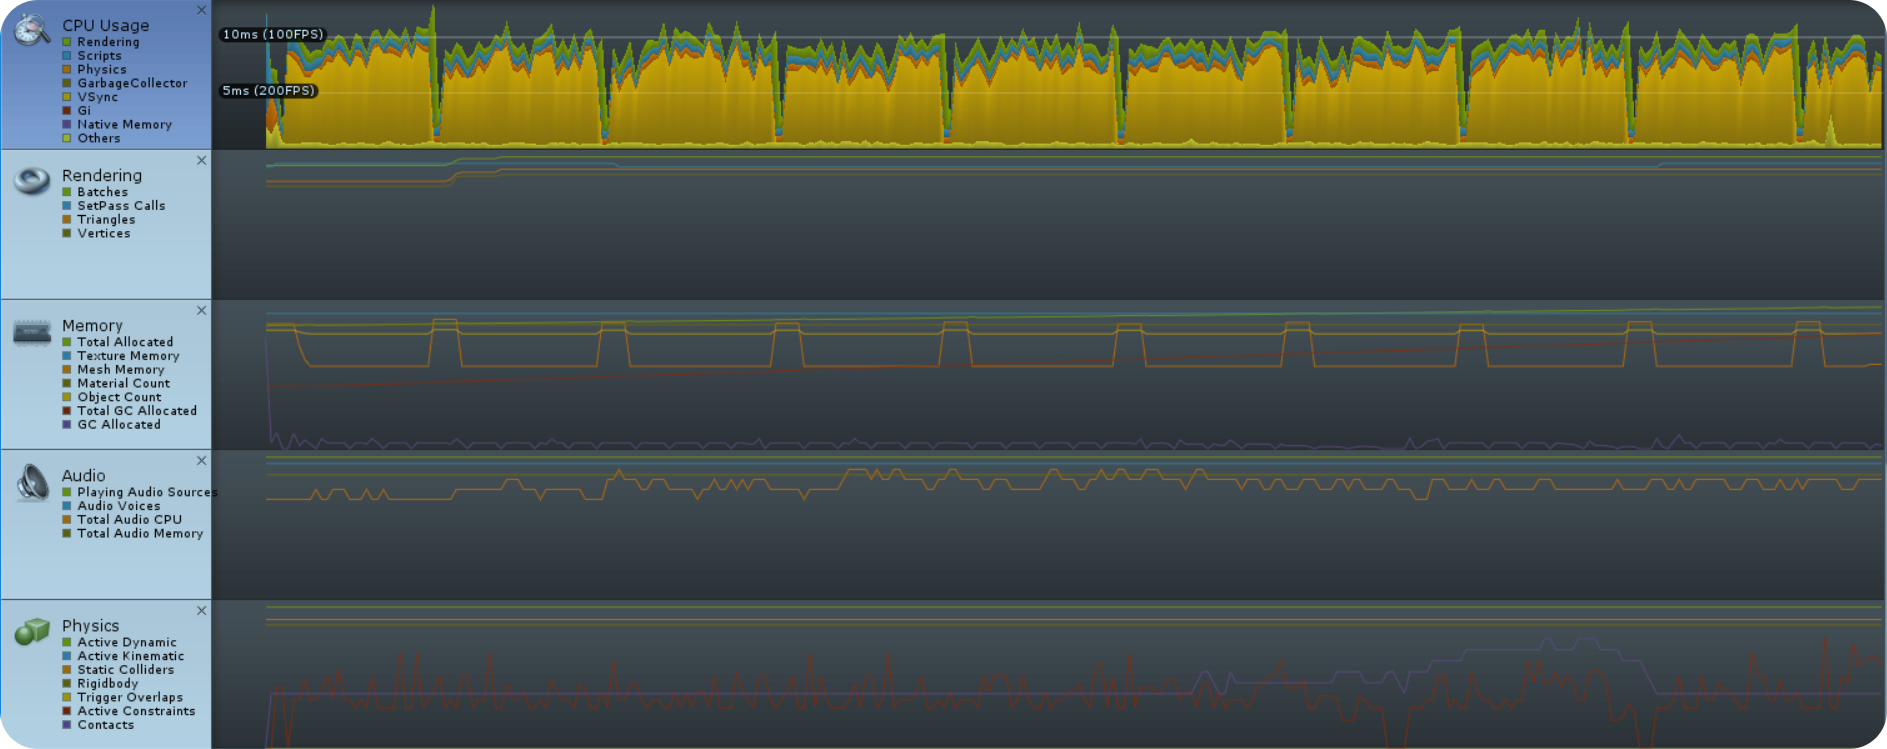
\includegraphics[width=0.9\textwidth]{profiling1_r.PNG}
      \caption{The profiler view of Unity\textsuperscript{\textregistered} Editor when a wine bottle rolls down a number of platforms.}
      \label{fig:profile}
\end{figure} 

When testing the limits of the tool, we found out that in Filter-based method a total of 16 objects can be active at the same time before audio gets distorted. The corresponding number for the Sinusoidal method is 12, since more calculations take place. Those numbers were obtained on the laptop mentioned above and using the \textit{Unity\textsuperscript{\textregistered} Audio Profiler window} and represent the amount of \textbf{``Playing Audio Sources''} without the \textbf{``Total Audio CPU''} exceeding $100\%$ (see figure \ref{fig:audio_profile}).

\begin{figure}[H]
  \centering
    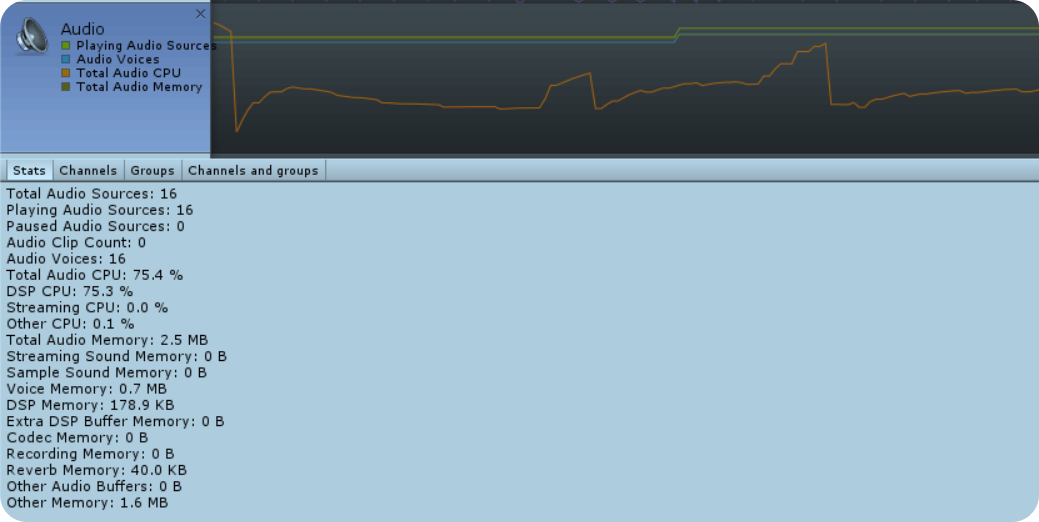
\includegraphics[width=0.9\textwidth]{audio_profile_r.PNG}
      \caption{The audio profiler view of Unity\textsuperscript{\textregistered} Editor when a total of 16 objects are enabled in the scene using the filter-based method for audio synthesis.}
      \label{fig:audio_profile}
\end{figure}

\subsection{How can we improve our work?}
\begin{itemize}
\item take into account the environment (reverberation etc)
\item make objects destructible
\item randomize initial phase so peaks of the sine wave don't line up and distort the sound (saturation)
\item spatialize at the same time with the synthesis
\item radiation and propagation (Interactive Acoustic Transfer Approximation for Modal Sound has a method)
Even though the recordings used to extract the modal data include information about the radiation and propagation of the sound in the environment, this thesis did not examine it.
\item use only one recording and interpolate for all areas
\item level of detail, using a masking threshold of e.g. 15dB as used in MEASUREMENTS OF PERCEPTUAL QUALITY OF CONTACT SOUND MODELS
\end{itemize}

\subsection{Pros and Cons of Procedural Game Audio}
pros\\
more adaptive (flexible/dynamic).\\
physics based.\\
possibility of alternations without extra memory.\\
less memory space.\\
no need for time consuming sound library development.\\
easy to create new sounds.\\
better for mobile platforms.\\

cons\\
usually bad quality (not realistic - you can tell it's synthesized).\\
more processing power.\\
additional code requirements.\\
not everyone is familiar with this sound design approach.\\
not every sound is easy to be produce procedurally.\\
